\documentclass[onecolumn,12pt]{article}

% packages to use/include
\usepackage{amsmath, amsthm, amssymb, amsfonts}
\usepackage{fullpage, graphicx, latexsym, enumitem}
\usepackage{color, xcolor, subfigure, wrapfig}
\usepackage{url, hyperref, authblk}

% definition of colours
\definecolor{dark-gray}{gray}{0.05}
\definecolor{skblue}{rgb}{0,0.08,0.45}

% First Page 
\title{\bf My First \LaTeX Article}
\author{SEC Student Name \thanks{\href{mailto:sec.student@gmail.com}{Email: sec.student@gmail.com}}}
\affil{Department of Physics, Asutosh College, Kolkata 700026, India}

\begin{document}
\flushbottom
\maketitle
\thispagestyle{empty}

\begin{abstract}
This is my first article in \LaTeX. I am a beginner in the world of \LaTeX.
I want to learn this cool document preparation software that has multifold benefits. Hence I perform my first try to create a latex template that contain some mathematical equations, tables, references and footnotes.  
\end{abstract}

\section{Introduction}
\label{intro}
Since the days I have learned to use a computer, I was inclined to learn a document preparation system and in the search, I had seen Microsoft Word in Windows and Libreoffice in Linux operating system. However I was looking for a better way of accountability of all the macros, citations, organization of the equations, tables. In the course of BSc at Asutosh College, I have been bestowed a Skill-enhancement Course by the Calcutta University where I am taking a course to learn Latex. This is my first LaTeX\cite{leslam} document. 

\section{Topics I must Learn}
\label{sec:1}
Here many things I'm determined to learn that I will initiate with a subsection.
\subsection{Enumerate \& Itemize}
\begin{enumerate}
\item Firstly, I am learning to enumerate such that I can put numbers other than bulltet points whenever required to highlight the key points I want to make. 
\item Secondly, there can be more topics that requires attention which comes only after I have placed the importance of the first item.
\end{enumerate}

\begin{itemize}
\item I am also learning to itemize different important topics that doesn't come sequelly and bullet points are absolutely good to highlight these points.
\item These points don't necessarily require some sequel to follow. It can be random.
\item[!] Hooray! I'm getting acquainted with LaTeX! I can call it a day!
\end{itemize}
\begin{enumerate}
	\item We can make the example of enumerate more complex as we want to make.
	\begin{enumerate}
	\item Just for example take this case where I only want to make a small point.
	\item At the same time I'm also making a relevant point related to the former.
	    \begin{enumerate}
	    \item Finally I decided to shut up!
	    \item I won't make another comment on this.
	    \item I mean really so. This is my last comment.
	    \end{enumerate}
	\end{enumerate}	
\end{enumerate}

\subsection{Paragraphs}
Now we will learn how to write paragraphs. It is not difficult at all. It just needs some practice to write, cite, refer the previous articles, books, resources {\it etc} to avoid plagiarism and to get a proper credit of your own work, for which you have determined to write this document. \\ \ \\
Basically we could do this just by using double backslash to separate out two paragraphs from one single chunk of writing. 
\paragraph{Paragraph with Suitable Heading:}
Suppose we want to define some quantity. So we can put a suitable heading and just define the corresponding subject without losing any generality of the text.

\subsection{Tables}
Making tables will be easier to play with, as you learn LaTeX. For example, let us try to make our first table \ref{tbl:param}: 

\begin{table}[h]
\small
\begin{tabular*}{1.0\textwidth}{@{\extracolsep{\fill}}|c|c|c|c|c|c|}
\hline
${\bf Observation}$ & $\Gamma$ & $\kappa$ & $\beta$ & $\zeta$ & $\eta$ \\
\hline
$1$ & $2.0$ & $10^{-3}$ & $-0.5$ & $2.67$ & $0.025$ \\
\hline
$2$ & $10^{-3}$ & $-0.75$ & $2.67$ & $0.01$ & $10^{-3}$ \\
\hline
$3$ & $0.99$ & $1.45$ & $2.67$ & $10^{-3}$ & $-0.75$ \\
\hline
$4$ & $2.5$ & $10^{-4}$ & $-0.75$ & $0.01$ & $0.99$ \\
\hline
$5$ & $1.5$ & $-0.25$ & $10^{-3}$ & $0.01$ & $1.45$ \\
\hline
$6$ & $10^{-2}$ & $2.0$ & $2.67$ & $10^{-3}$ & $0.99$ \\
\hline
\end{tabular*}
\caption{\label{tbl:param} Values of parameters.}
\end{table}

\subsection{Mathematical expressions}
To demonstrate the idea, let us revisit how timescale varies with mass and length in different commonly encountered systems. 
\subsubsection{Linear Harmonic Oscillator}
The governing equation is 
\begin{equation}
\label{eq:lho}
\boxed{m \frac{d^2x}{dt^2} + kx = 0}, 
\end{equation}
where $k$ is the spring's constant. The natural frequency of the system is\footnote{This is because a general solution is of the form $x = Ae^{i(\omega t \pm \phi)}$ where $A$ is amplitude, $\omega$ is the angular frequency and $\phi$ is the phase.} 
$\omega_0 = \sqrt{k \over m}$. This yields the time scale $\tau_0 \sim \sqrt{\frac{m}{k}}$.

\subsubsection{Wave Equation}
For a plane propagating wave along $x-$direction, the equation takes the form
\begin{equation}
\label{eq:we}
\boxed{\ddot{u} = v^2 \nabla^2 u}, 
\end{equation}
where the natural frequency, unlike eqn.(\ref{eq:lho}), of the system is\footnote{This can be realized taking the form of the wave $u = Be^{i(\omega t-{\bf k}\cdot {\bf r})}$ where $B$ is the amplitude, $\omega$ is the angular frequency and $k$ is the wavevector of the wave.} $\omega_0 = \pm vk$ where $k = 2\pi/\lambda$. This yields the time scale $\tau_0 \sim {\lambda \over v}$.

\subsubsection{Diffusion Equation}
In case of say heat diffusion happening along $x-$direction, the heat equation reads
\begin{equation}
\label{eq:de}
\boxed{\dot{u} = \mathcal{D} \nabla^2 u}, 
\end{equation}
where taking the Fourier transform yields for the natural frequency, unlike eqn.(\ref{eq:lho},\ref{eq:we}), of the system as $-i\omega_0 = \mathcal{D} k^2$. This results into $\tau_0 \sim {\lambda^2 \over \mathcal{D}}$.

\subsubsection{Basis Set}
For any continuous and differentiable function $f$ varying in space and time, we can separate the variables of the function by going to principal axes ${\bf \hat{i}}, {\bf \hat{j}}, {\bf \hat{k}}$ in the rectangular coordinate system. Since the Spherical Harmonics form a complete basis of orthonormal functions,
$f$ can be expanded as,
\begin{equation}
f({\bf x},{\bf \hat{n}},t) = \sum_{i=0}^{\infty} g_i({\bf x},t) Y^i({\bf \hat{n}}), 
\end{equation}
where $g_i({\bf x},t)$ are the expansion coefficients and $Y^i({\bf \hat{n}})$ are the spherical harmonics, that we perform multiple expansion to yield, 
\begin{equation}
f({\bf x},{\bf \hat{n}},t) = \frac{1}{4\pi} \large[1 + 
\underbrace{{\bf \hat{n}} \cdot {\bf P}({\bf x},t)}_{Dipole} 
+ \overbrace{[{\bf \hat{n}}_\alpha \otimes {\bf \hat{n}}_\beta] {\bf Q}_{\alpha\beta}({\bf x},t)}^{Quadrupole} 
+ \underbrace{\cdots}_{Octupole, Hexadecapole, \cdots} \large].
\end{equation}
where, 
\begin{eqnarray}
1 &=& \int d{\bf \hat{n}} f({\bf x},{\bf \hat{n}},t), \\
{\bf p}({\bf x},t) &=& \int d{\bf \hat{n}}~ {\bf \hat{n}} f({\bf x},{\bf \hat{n}},t), \\
{\bf Q}({\bf x},t) &=& \int d{\bf \hat{n}}~ [{{\bf \hat{n}}\otimes{\bf \hat{n}}}] ~f({\bf x},{\bf \hat{n}},t).
\label{nemord}
\end{eqnarray} 

\subsection{Inscribing Figure \& Text}
\begin{wrapfigure}{l}{0.4\textwidth}
	\centering
	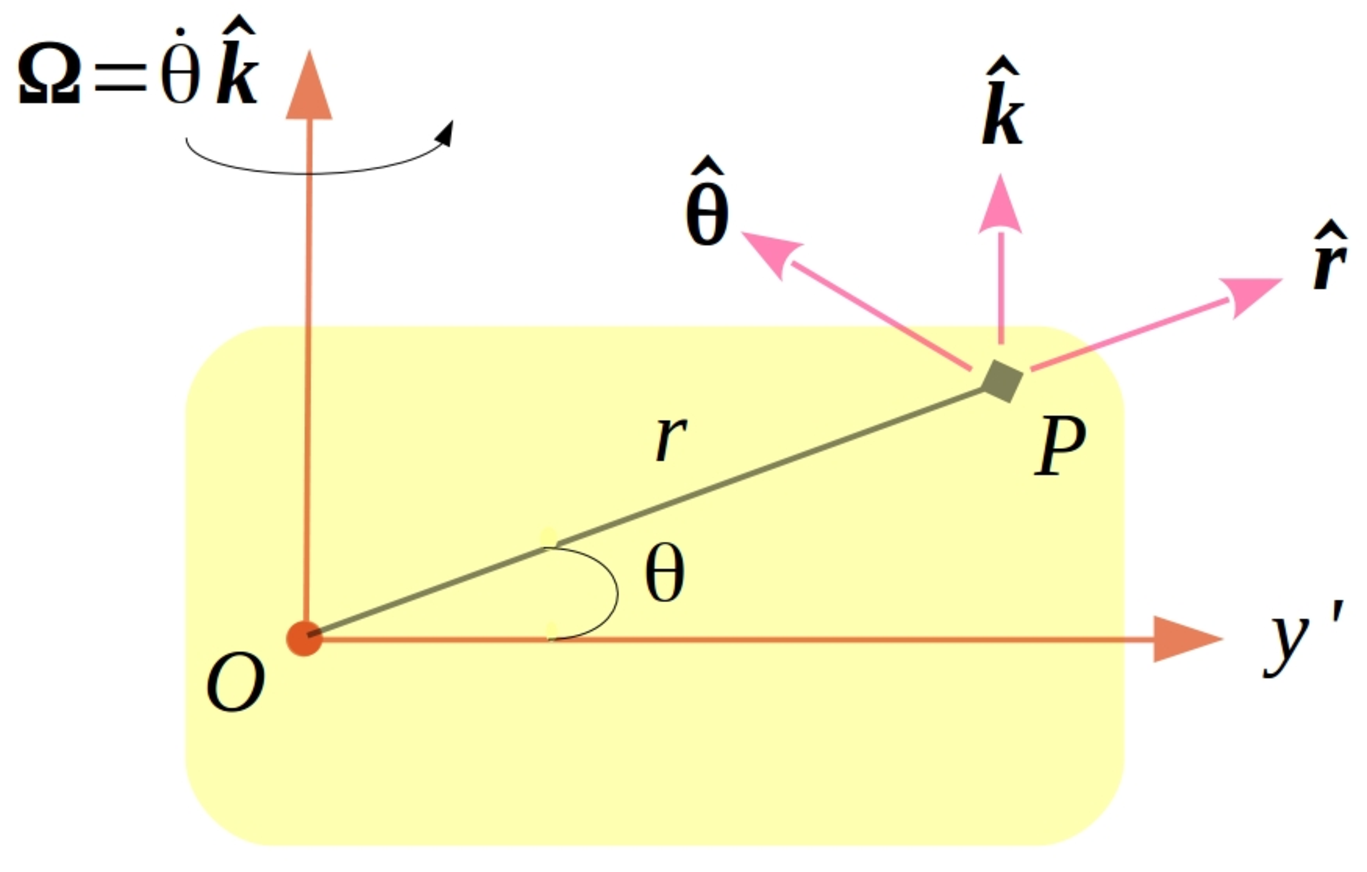
\includegraphics[width=2.5in, height=1.6in]{/home/amit/Documents/Books/Teaching/Asutosh/Mechanics/rot.pdf}
\end{wrapfigure} 
In figure beside, the polar coordinates $(r,\theta)$ are measured relative to an inertial frame $\mathcal{F}$, 
while $\mathcal{F}^\prime$ is a frame rotating about the $z$-axis passing through $\mathcal{O}$ with angular 
velocity ${\mathbf\Omega}$. By using the velocity and acceleration transformation formula between inertial 
and rotating coordinate system, it can be shown that
\textbf{ \begin{center}
		$\displaystyle{  
			{\bf v} = {\dot r}{\bf \hat{r}} + r{\dot \theta}{\boldsymbol{\hat{\theta}}}; ~~
			{\bf a} = ({\ddot r} - r{\dot \theta}^2){\bf \hat{r}} + (r{\ddot \theta} + 2{\dot r}{\dot \theta}){\boldsymbol{\hat{\theta}}} }$.
\end{center}}.
\newline
\begin{figure*}[ht]
	\centering
	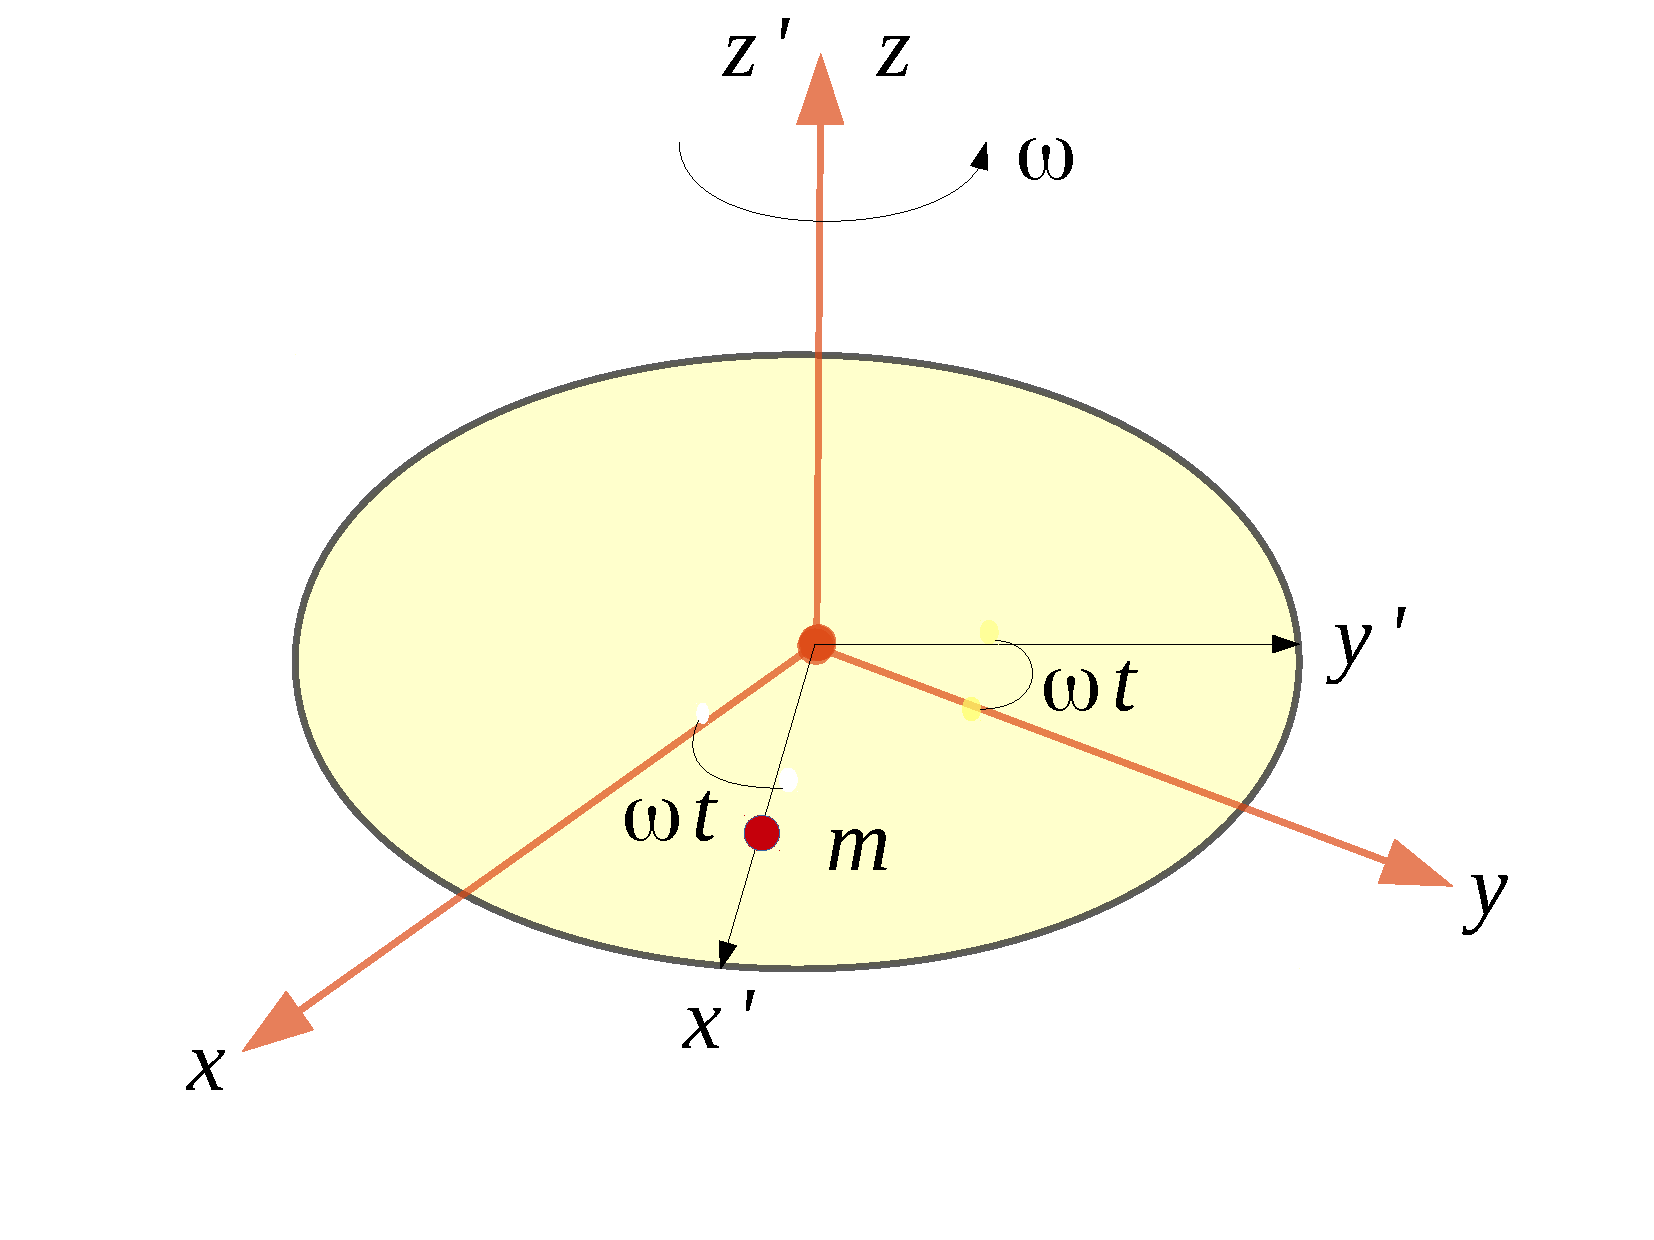
\includegraphics[width=2.6in, height=2.2in]{/home/amit/Documents/Books/Teaching/Asutosh/Mechanics/bug.pdf}
	\caption{A turn-table marked with three orthogonal axes $(x^\prime,y^\prime,z^\prime)$ is rotating on the Earth, assumed to be an inertial frame $(x,y,z)$, with constant angular velocity ${\boldsymbol \omega}$ about $z$-axis. At $t=0$, both frames coincide with each other. A ball of mass $m$ is rolling outward without slipping along the $x^\prime$-axis with a constant velocity $v$.}
\end{figure*}

But now suppose, I do not want to wrap the text but want to display a fullscape figure and the accompanying text just below it. 
This can be demonstrated with the help of includegraphics within the graphics package. Note that this is not limited to pdf pictures only.


\section{Conclusion \& Inferences}
This section will be devoted as a small summary of the main results in a nutshell as well as future direction of the presented study. This is like winding up the article, paper, project or the relevant document you are preparing.

\bibliographystyle{plain}  
%\bibliographystyle{acm}  % comment out different bib styles that suits.
%\bibliographystyle{apalike}
%\bibliographystyle{ieeetr}
%\bibliographystyle{alpha}
%\bibliographystyle{siam}
%\bibliographystyle{unsrt}
\bibliography{references}
\end{document}
